% Set this figure's name when externalised 
\tikzsetnextfilename{contour-integral} 
%
%%%%%%%%%%%%%%%%%%%%%%%
%%%% BLACK MAGIC  %%%%%
%%%% DO NOT TOUCH %%%%%
%%%%%%%%%%%%%%%%%%%%%%%
\usetikzlibrary{decorations.pathreplacing,decorations.markings}
%
\tikzset{
  % style to apply some styles to each segment of a path
  on each segment/.style={
    decorate,
    decoration={
      show path construction,
      moveto code={},
      lineto code={
        \path [#1]
        (\tikzinputsegmentfirst) -- (\tikzinputsegmentlast);
      },
      curveto code={
        \path [#1] (\tikzinputsegmentfirst)
        .. controls
        (\tikzinputsegmentsupporta) and (\tikzinputsegmentsupportb)
        ..
        (\tikzinputsegmentlast);
      },
      closepath code={
        \path [#1]
        (\tikzinputsegmentfirst) -- (\tikzinputsegmentlast);
      },
    },
  },
  % style to add an arrow in the middle of a path
  mid arrow/.style={postaction={decorate,decoration={
        markings,
        mark=at position .5 with {\arrow[#1]{stealth}}
      }}},
}
%%%%%%%%%%%%%%%%%%%%%%%
%%%%%%%%%%%%%%%%%%%%%%%
%%%%%%%%%%%%%%%%%%%%%%%
%%%%%%%%%%%%%%%%%%%%%%%

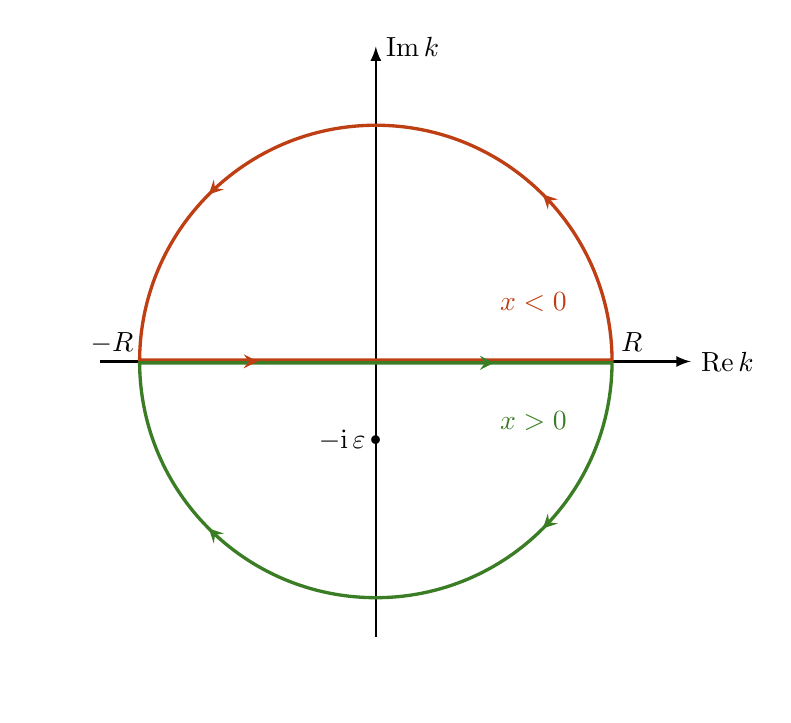
\begin{tikzpicture}[thick]
    % axes and points
    \draw
      (-3.5,0) edge[-latex] node[at end,right]{${\rm Re}\,k$} (4,0) %Horizontal axis
      (0,-3.5) edge[-latex] node[at end,right]{${\rm Im}\,k$} (0,4) %Vertical axis
      
      %Ensure symmetric borders
      (-4,+0) node(phantomx) {\phantom{${\rm Re} k$}}
      (+0,-4) node(phantomy) {\phantom{${\rm Im} k$}}
      
      (0,-1) node[scale=3](-i){.} node[left]{$-{\rm i}\,\varepsilon$} %Pole

      % For the circles
      (3,0)  coordinate(R) node[below]{}
      (-3,0) coordinate(-R) node[below]{}

    % For the shifted straight lines
      (+3,+0.0175)  coordinate(UpperR) node[below]{}
      (+0,-0.0175)  coordinate(UpperZero) node[below]{}
      (-3,+0.0175) coordinate(-UpperR) node[below]{}
      (+3,-0.0175)  coordinate(LowerR) node[below]{}
      (+0,-0.0175)  coordinate(LowerZero) node[below]{}
      (-3,-0.0175) coordinate(-LowerR) node[below]{}

    %% For labels
      (3.25,0.5) node[below]{$R$}
      (-3.35,0.5) node[below]{$-R$}

      (+2.0,+0.5) node[above]{\textcolor{Bittersweet}{$x<0$}}
      (+2.0,-0.5) node[below]{\textcolor{OliveGreen}{$x>0$}}
    ;
    % the path
    
    % Upper arc
    \draw[Bittersweet, very thick]
    (-R) arc(+180:+0:3cm)
    (-UpperR) -- (UpperR)
    ;
    
    %lower arc
    \draw[OliveGreen, very thick]
    (-R) arc(-180:+0:3cm)
    (-LowerR) -- (LowerR)
    ;

    %Upper Contour Arrows
    \path [Bittersweet, very thick,postaction={on each segment={mid arrow=Bittersweet}}]
    (R) arc(+0:+180:3cm)
    (-UpperR) -- (UpperZero)
    ;

    %Lower Contour Arrows
    \path [OliveGreen, very thick,postaction={on each segment={mid arrow=OliveGreen}}]
    (R) arc(+0:-180:3cm)
    (LowerZero) -- (LowerR) 
    ;

\end{tikzpicture}
